\section{Introduction}

\begin{enumerate}
	\item show airfoil
	\item table of freestream conditions and Re
	\item xfoil estimates of:
	\begin{itemize}
		\item max  L/D ratio, and AoA at which this occurs
		\item max $C_l$, and AoA at which this occurs
		\item Note: take both of the above directly from airfoiltools.com, at the closest reynolds number available
	\end{itemize}
\end{enumerate}

\begin{figure}[h!]
	\centering
	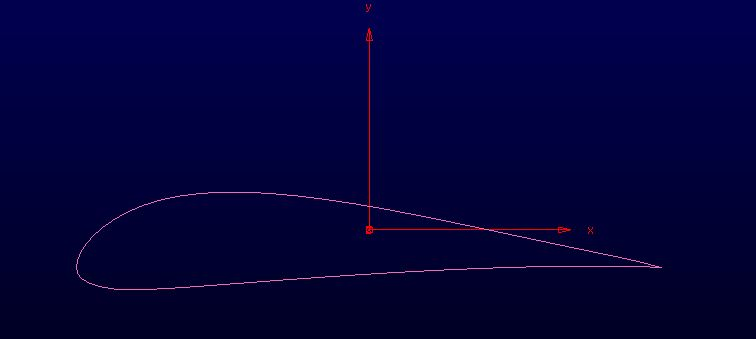
\includegraphics[width=\textwidth]{general_images/airfoil_image}
	\caption{Eppler 1210 Airfoil shown in Pointwise}
\label{fig:universe}
\end{figure}

\begin{table}[]
\caption{Operating conditions for all cases}
	\centering
	\begin{tabular}{|r|r|} \hline
		Quantity & Value \\ \hline \hline
		Pressure & 103,000 Pa \\ \hline
		Temperature & 298 K  \\ \hline
		Velocity & 17.88 ms$^{-1}$ \\ \hline
		Viscosity & 1.789e-05 kgm$^{-1}$s$^{-1}$ \\ \hline
		Re \# & 1,224,315 \\ \hline
	\end{tabular}
\end{table}

\begin{table}[]
\caption{XFoil Predictions, Re = 1e9, ncrit = 9}
	\centering
	\begin{tabular}{|r|r|r|} \hline
				& Value	& AoA \\ \hline \hline
		Max L/D & 117.1309 & 8 \\ \hline
		Max $C_L$ & 1.8542 & 16 \\ \hline	
	\end{tabular}
\end{table}

% gradient: least squares cell based
% pressure: second order
% momentum: second order upwind
% turbulent kinetic energy: first order upwind
% specific dissipation rate: first order upwind
% intermittency: first order upwind
% momentum thickness Re: first order upwind

%\begin{figure}[h!]
%\centering
%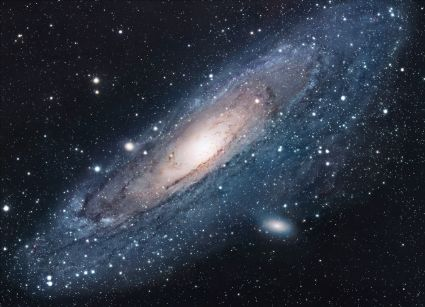
\includegraphics[scale=1.7]{universe}
%\caption{The Universe}
%\label{fig:universe}
%\end{figure}
